There  are  arguably  few  places  in  the  world  that  can  claim  a biodiversity as high as Colombia’s. Colombia’s unique ecosystem is comprised of numerous animal species that have adapted to a diverse set of habitats. Among these, weakly electric fish make up \~80\%  of the biomass of the respective native fish fauna \citep{marrero1991notas}. The south American weakly electric fish belong to the order of Gymnotiformes, with five known families and 135 different species (current state \citeyear{albert2005diversity}, \citeauthor{albert2005diversity}).

The weakly electric fish evolved an electric organ which cells discharge simultaneously and create an electric field around the animal \citep{Zupanc_Bullock_2005}. They use this electric organ discharge (EOD) for electrolocation, orientation and object recognition \citep{Heiligenberg_73}, communication \citep{Hopkins_74} and foraging \citep{Nelson_MacIver_1999}. Amongst the weakly electric fish two types of EOD are known. Wave-type fish emit a continuous, quasi sinusoidal EOD with a constant frequency, while pulse-type fish emit very brief stereotyped pulses, with varying inter-pulse-intervals \citep{Zupanc_Bullock_2005}.
The electric organ discharge is 
not only different between these two types, it also differs between species, i.e. in their waveforms and their EOD frequencies \citep{Zupanc_Bullock_2005}.
% about ecletric organ and how it represents the dominance in males (A.apteronotus)
Also differences in EOD frequency between individuals of the same species can be found. This differences in frequency are known as indicating dominance among males \citep{HAGEDORN1985}.\\

\begin{figure}
    \centering
    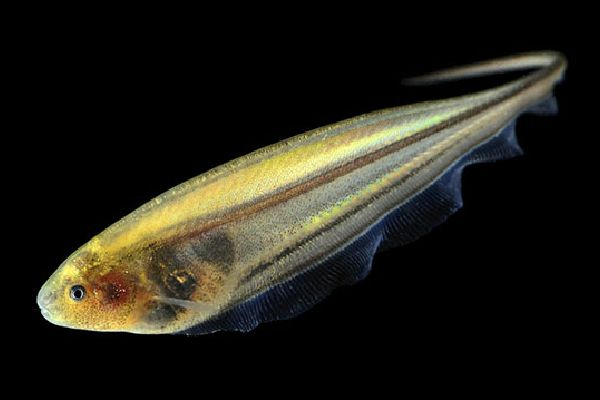
\includegraphics[width = \textwidth]{pictures/Eigenmannia_virescens.jpg}
    \caption{\textbf{Eigenmannia virescens.} Picture of a cute weakly electric fish of the species \textit{Eigenmannia virescens} from a questionable, Russian webside: \url{http://aquavitro.org/2014/11/13/vidy-ryb-nozhej/}.}
    \label{fig:eigenmannia_cute}
\end{figure}

Previous studies have shown that dominance strongly influences the inhabitation of shelters \citep{raab2019}.
Which is relevant for the animal's survival, since weakly electric fish hide during the day \citep{Hopkins_74}.     
In staged laboratory settings it could be shown that dominant males, with the highest EOD frequencies, defend the best shelters against subordinate males \citep{raab2019}.
It could also been shown that, at least for some species, male individuals are more likely to defend their shelters against same sex conspecifics. In contrast, females are more likely to share shelters with their conspecifics \citep{dunlap2002retreat}.
A relation between shelter, or more general habitat selection, was also already shown for other species within the animal kingdom, i.e. aquatic species like salmons \citep{redsalmon1995}, but also in terrestrial species, like redstarts \citep{sherry1989redstarts} or lizards \citep{downes1998heat}.
In general it is known, that different species prefer different habitats. However, for each species the preferred or most attractive habitat can depend on other characteristics.
In case of weakly electric fish, some species prefer to seek shelter between roots (Eigenmannia, \citeauthor{Hopkins_74}, \citeyear{Hopkins_74}), under sunken rocks Gymnotus, \citeauthor{westby1988ecology}, \citeyear{westby1988ecology}), in leaf litter (Brachyhypopomus, \citeauthor{hagedorn1988ecology}, \citeyear{hagedorn1988ecology}) or even in sand (Gymnorhamphichthys, \citeauthor{lissmann1965activity}, \citeyear{lissmann1965activity}).
For aquatic species, the most attractive habitat can also depend on water flow or water depth \citep{aadland1993stream}.
% was wir getan haben und warum
While gymnotiform weakly electric fish are well researched in the lab and their dominance behaviour as well, much less is known about the ecology and ethology of these animals in the wild. 
Therefore, first conditions of their natural habitat in the LLanos of the Orinoco basin, in the Reserva el Caduceo in San Martin, Meta, Colombia were characterised. 
Second, the occurring species of Gymnotiformes, \textit{Apteronotus macrostomus, Eigenmannia virescens} and gymnotiform pulsefish, and their density in these habitats were sampled.
Between the species, their occurrence densities, dependent on the habitat characteristics, were compared in order to detect possible habitat preferences.
Additionally, for the species \textit{A. macrostomus} the EOD frequency, which is correlated with dominance, was compared within the inhabited habitats. Since, dominance between territorial males might not only determine their fitness but might also influence selection of resting sites, because better resting sites might reduce physiological costs.
Summarised, our research questions were:\\

\begin{itemize}
\item[1.] What are the environmental conditions (ground conditions, water flow and depth) of the natural habitat of gymnotiform weakly electric fish?

\item[2.] Do different species of weakly electric fish prefer different habitats conditions?

\item[3.] Does the social dominance influences the  habitat selection in \textit{A. macrostomus}?
\end{itemize}{}
